% -*- TeX-engine: luatex; fill-column: 72; eval: (auto-fill-mode -1); eval: (visual-fill-column-mode 1); eval: (visual-line-mode 1); eval: (adaptive-wrap-prefix-mode 1) -*-
\documentclass[12pt]{article}
\usepackage{ttr}
\usepackage[colorlinks=true,allcolors=blue]{hyperref}
% \hypersetup{
%   colorlinks   = true, 
%   urlcolor     = darkblue,
%   linkcolor    = darkblue,
%   citecolor    = darkblue
% }
\usepackage{graphicx}
\usepackage{booktabs}
\usepackage{siunitx}

% \usepackage[english]{babel}
% \input{styles}
% \title{
% The Alan Turing Institute - 
% Carbon Emissions from Computing}
% \author{Rosie Wood}
% \date{September 2025}
% \affil{The Alan Turing Institute}
\newcommand{\cooe}{\ensuremath{\mathrm{CO}_2\mathrm{e}}}
\newcommand{\mtcooe}[1]{\qty[qualifier-mode=combine]{#1}{\mega\tonne\of{\cooe}}}
\newcommand{\tcooe}[1]{\qty[qualifier-mode=combine]{#1}{\tonne\of{\cooe}}}
\DeclareSIUnit\KWH{kWh} % to keep the kW with the h
\DeclareSIUnit\GPUh{GPU\,h} % because
\newcommand{\gcookwh}[1]{\qty[qualifier-mode=combine, per-mode=symbol]{#1}{\gram\of{\cooe}\per\KWH}}
\newcommand{\eg}{\emph{e.g.}}
\newcommand{\ie}{\emph{i.e.}}
%
\usepackage[sorting=none]{biblatex}
\addbibresource{bibliography.bib}
%
\begin{document}
\setcounter{page}{3}
% \maketitle

% \setcounter{tocdepth}{1}
% \tableofcontents
% \newpage

\section{Introduction}
\label{sec:intro}

In 2024, data centres accounted for around \qty{1.5}{\percent} of the world’s electricity consumption and around \mtcooe{180} of greenhouse gas emissions~\cite{iea_energy_ai} --- around \qty{0.3}{\percent} of total global greenhouse gas emissions~\cite{unep_egr_2025}.
This number is forecast to more than double by 2030, largely driven by AI~\cite{iea_energy_ai}.

In this work, we estimate the greenhouse gas emissions from the Turing's use of its main compute resources: Microsoft Azure, UK High Performance Computing systems (HPCs) and GitHub Actions, and identify areas in which we could reduce these emissions. Our results are summarised in Table~\ref{tab:summary_table}.

\begin{table}[ht!]
  \centering
  \caption{Summary of operational and embodied emissions from Azure, HPC and GitHub Actions between September 2024--August 2025.}
  \label{tab:summary_table}
  \begin{tabular}{@{}rrrrr@{}}\toprule
    Compute resource  & \shortstack{Electricity\\/ kWh} & \shortstack{Total\\/ t\cooe} & \shortstack{Operational\\/ t\cooe} & \shortstack{Embodied\\/ t\cooe}\\\midrule
    Microsoft Azure       &    N/A &  2.9 &   $0^{\dag}$ & 2.9 \\
    Baskerville HPC (CHP) & 83{,}300 &  31  &  25          & 6   \\
    GitHub Actions        & 380$^{\ddag}$ &  0.1 &   $0^{\dag}$ & 0.1 \\ \bottomrule
  \end{tabular}
  \smallskip\\
  \noindent$^{\dag}$\,Market-based operational emissions; location-based emissions cannot be calculated (see Section~\ref{sec:azure}).\\
  \noindent$^{\ddag}$\,Extrapolated from six months of data (March--August 2025).
\end{table}

To help put these emissions from computing into perspective it can be helpful to compare against carbon emissions from other sources on similar scales:

 \begin{itemize}
     \item In the UK in 2022, per-capita emissions were approximately \tcooe{5} per year~\cite{iea_uk_emissions}.
     \item A flight\footnote{For details on the methodology used to calculate the emissions from the flights see  \url{https://www.myclimate.org/en/information/about-myclimate/downloads/flight-emission-calculator/}.} from London (LHR) to:
     \begin{enumerate}
         \item Madrid (MAD) emits approximately \tcooe{0.308} per passenger~\cite{co2_flights},
         \item New York (JFK) emits approximately \tcooe{0.978} per passenger~\cite{co2_flights},
         \item Melbourne (MEL) via Kuala Lumpar (KUL) emits approximately \tcooe{3.4} per passenger~\cite{co2_flights}.
     \end{enumerate}
 \end{itemize}

The remainder of this report is structured as follows. Section~\ref{sec:background} provides background on emissions scopes and methodology. Section~\ref{sec:azure} covers emissions from the Turing's use of cloud computing (primarily Microsoft Azure), Section~\ref{sec:hpc} covers emissions from our use of HPC systems (primarily Baskerville) and Section~\ref{sec:github} covers emissions from GitHub Actions. Finally, we summarise our findings and outline potential areas for reducing emissions.

\section{Background}
\label{sec:background}

Emissions are categorised as one of three scopes~\cite{nationalgrid}:

\begin{description}
    \item[Scope 1] covers emissions from sources that an organisation owns or controls directly.
    \item[Scope 2] are emissions that a company causes indirectly and come from where the energy it purchases and uses is produced. Scope 2 emissions can be calculated in one of two ways:
    \begin{itemize}
        \item Market-based Scope 2 emissions reflect those from electricity that companies have purposefully chosen (\eg, if they have chosen a fully renewable tariff, market-based Scope 2 emissions will be zero).
        \item Location-based Scope 2 emissions reflect the average emissions intensity of grids on which energy consumption occurs.
    \end{itemize}
    \item[Scope 3] encompasses emissions that are not produced by the company itself and are not the result of activities from assets owned or controlled by them, but by those that it is indirectly responsible for up and down its value chain.
\end{description}

Emissions from compute broadly come from one of two sources: emissions from energy consumption when running the hardware (known as operational emissions) and embodied emissions from manufacturing, transporting and disposing of the hardware. For the compute provider (\eg, Azure or an HPC host organisation), operational emissions correspond to Scope~1 (on-site fuel use) and Scope~2 (purchased electricity), while embodied emissions fall under Scope~3 (upstream/downstream supply chain). For the Turing, the vast majority of our emissions from computing are classed as Scope~3 since in most cases we do not own the hardware we run on nor do we pay directly for the electricity that powers it. Emissions from Turing-owned hardware (\eg, laptops, commercial GPUs and Raspberry Pis) are not covered in this report, though these may become increasingly significant with the growing use of locally-run LLMs.

To calculate operational emissions, the carbon emissions from electricity use are calculated by multiplying energy consumption by the carbon intensity of that energy, where carbon intensity is a measure of the carbon emissions per kWh of electricity consumed. This is a relatively simple calculation and makes it straightforward to estimate operational emissions provided that energy consumption and carbon intensity are known. Embodied emissions, however, are far more complicated to calculate since they require upstream data from vendors, such as manufacturing and transportation emissions, and a life-cycle assessment.

\section{Cloud}
\label{sec:azure}

\subsection{Microsoft Azure}

Microsoft Azure has its own carbon optimisation and emission tracking dashboard which make it possible to view emissions resulting from the Turing's Azure usage. Azure users can access this themselves and see data related to Azure subscriptions they are part of. An example screenshot is shown in Figure \ref{fig:azure_dashboard} (note that this shows data for different dates than discussed below).
\begin{figure}[!ht]
    \centering
    \includegraphics[width=1\linewidth]{azure_dashboard.png}
    \caption{Azure Carbon Optimisation dashboard}
    \label{fig:azure_dashboard}
\end{figure}

The Azure emissions dashboard breaks down emissions by month and by scope. Here, Scope~1 emissions refer to Microsoft's Scope~1 emissions (\eg, from their own power plants), Scope~2 emissions refer to Microsoft's Scope~2 emissions (\eg, from energy they buy from the grid) and Scope~3 emissions refer to Microsoft's Scope~3 emissions (\eg, from the hardware they purchase).

Figure~\ref{fig:azure_monthly} shows the data for the past year (September 2024--August 2025). From this, we see the majority of the Turing's Azure emissions come from Microsoft's Scope~3 emissions, with a small contribution from Microsoft's Scope~1 emissions (most likely back-up power generation). Over this period, the Turing's total emissions from Azure were just \tcooe{2.9}.

This number is surprisingly low because Scope~2 emissions, which we would expect to be the biggest contributor to Azure emissions, are reported as zero. That is because Microsoft only report market-based Scope~2 emissions, which reflect the carbon intensity of the specific energy tariff they have chosen rather than the grid average (as described in Section~\ref{sec:background}), and since Microsoft uses renewable energy tariffs~\cite{azure_docs_scope2}; the carbon intensity of their energy is zero. Since there is no information on our energy usage, it is impossible to calculate location-based Scope~2 emissions.

\begin{figure}[!ht]
    \centering
    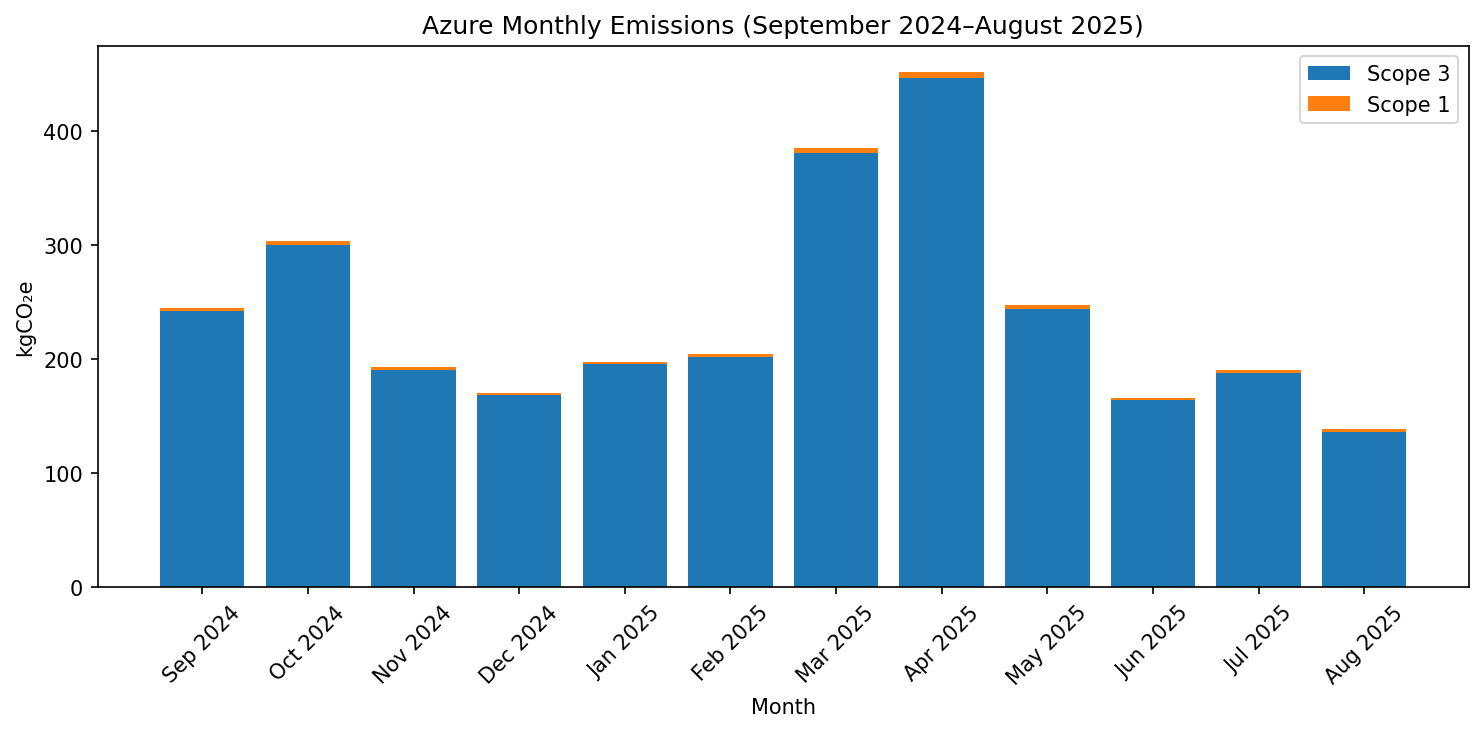
\includegraphics[width=0.75\linewidth]{azure_monthly.png}
    \caption{Azure monthly emissions (September 2024--August 2025)}
    \label{fig:azure_monthly}
\end{figure}

\section{HPC}
\label{sec:hpc}

\subsection{Baskerville}

Baskerville is by far the most widely used HPC at the Turing due to our institutional allocation which makes it particularly easy for Turing projects to access and utilise Baskerville HPC. Consequently, it is also our biggest source of compute emissions.

Baskerville is hosted by the University of Birmingham which, based on information from the Baskerville team, uses a gas powered combined heat and power (CHP) plant to power its campus. Consequently, Baskerville's operational emissions should be calculated using the carbon intensity of this CHP plant instead of that of the national grid.
There is limited information about emissions from Birmingham's CHP plant, but the University of Edinburgh reported its CHP plant emissions had a carbon intensity of \gcookwh{366}~\cite{edi_chp}---almost three times higher than the UK national average of \gcookwh{124}~\cite{average_ci_2024} in~2024. 
Noussan \emph{et al.}\ also found similar values, suggesting an annual average in the range \qtyrange[qualifier-mode=combine,range-units=single,per-mode=symbol]{270}{304}{\gram\of{\cooe}\per\KWH}~\cite{NOUSSAN2024}. We have therefore used a value of \gcookwh{300} to represent the estimated carbon intensity of the University of Birmingham's CHP plant.

As Turing admins for Baskerville, we are able to access an admin portal to download usage data for the whole Turing across all time.
This data contains somewhat limited information for each job, but includes run times, requested resources and submission dates. 
This is enough information to be able to create a rough estimate for operational emissions originating from the Turing's usage of Baskerville.

The code in the turing\_emissions repository\footnote{\url{https://github.com/rwood-97/turing_emissions/tree/main}} shows a simple way of calculating operational emissions from our Baskerville usage.
This is done using the formula shown in Equation \eqref{eq:emission1}
% for example $E_{\text{gpu}}$
where $E_{\text{gpu}}$, $E_{cpu}$ and $E_{mem}$ are the energy used by
the GPUs, CPUs and memory, respectively, PUE is the power usage
effectiveness of the HPC and CI is the carbon intensity at the time of
that energy usage.  Energy is calculated using
equation~\eqref{eq:energy1} where $E_\text{component}$ is the energy used by
the component (GPU, CPU or memory), $t_\text{component}$ is the time that
component is in use for and $P_\text{component}$ is the power draw of that
component.  For both GPU and CPU, power draw can be taken as the Thermal
Design Power (TDP) of the component, as reported by the manufacturer,
and for memory, power draw can be taken as a constant power draw of
\qty{0.3725}{\watt\per\giga\byte} of requested
memory~\cite{green_algorithms}.

\begin{equation}
E_{\text{operational}} = (E_\text{gpu} + E_\text{cpu} + E_\text{mem}) \times \text{PUE} \times \text{CI}
    \label{eq:emission1}
\end{equation}

\begin{equation}
    E_\text{component} = t_\text{component} \times P_\text{component}
    \label{eq:energy1}
\end{equation}

Figure~\ref{fig:baskerville_energy} shows the calculated energy usage of Turing's Baskerville jobs since mid-2021 (when the Turing first gained pilot access to Baskerville), broken down by year and component. Here we see that energy consumption is dominated by GPU and CPU usage whilst memory accounts for a comparatively smaller fraction.

Although these calculated energy values should only be taken as estimates due to large errors in the data, they are accurate enough to give a sense of our energy usage over the years.
Errors originate from the following sources:
\begin{itemize}
    \item The energy values shown reflect the energy needed to operate GPUs, CPUs and memory, as well as the overheads of the Baskerville HPC facility. However, they do not take into account additional overheads, such as energy needed to operate interconnect switches, storage, coolant systems, etc. For ARCHER2, the UK National Supercomputing Service hosted by EPCC at the University of Edinburgh, these overheads account for around \qty{15}{\percent} power draw~\cite{archer2_scope2} and for Isambard-AI, an AI-optimised HPC and part of the UK's AI Research Resource, these overheads account for around \qty{8}{\percent} of operational emissions~\cite{grace_hpc}. This would mean the values are underestimating the energy requirements for running Baskerville.
    \item The energy values shown are calculated using the thermal design power (TDP) values provided by NVIDIA for their GPUs and therefore assume \qty{100}{\percent} GPU power usage. However, GPU utilisation is often less than \qty{100}{\percent} when running GPU jobs on HPC~\cite{gpu_utilisation} and, in fact, according to the Baskerville team, some of the Baskerville GPUs are power capped. This would mean the values are overestimating the energy requirements when using Baskerville GPUs.
\end{itemize}

\begin{figure}[ht!]
    \centering
    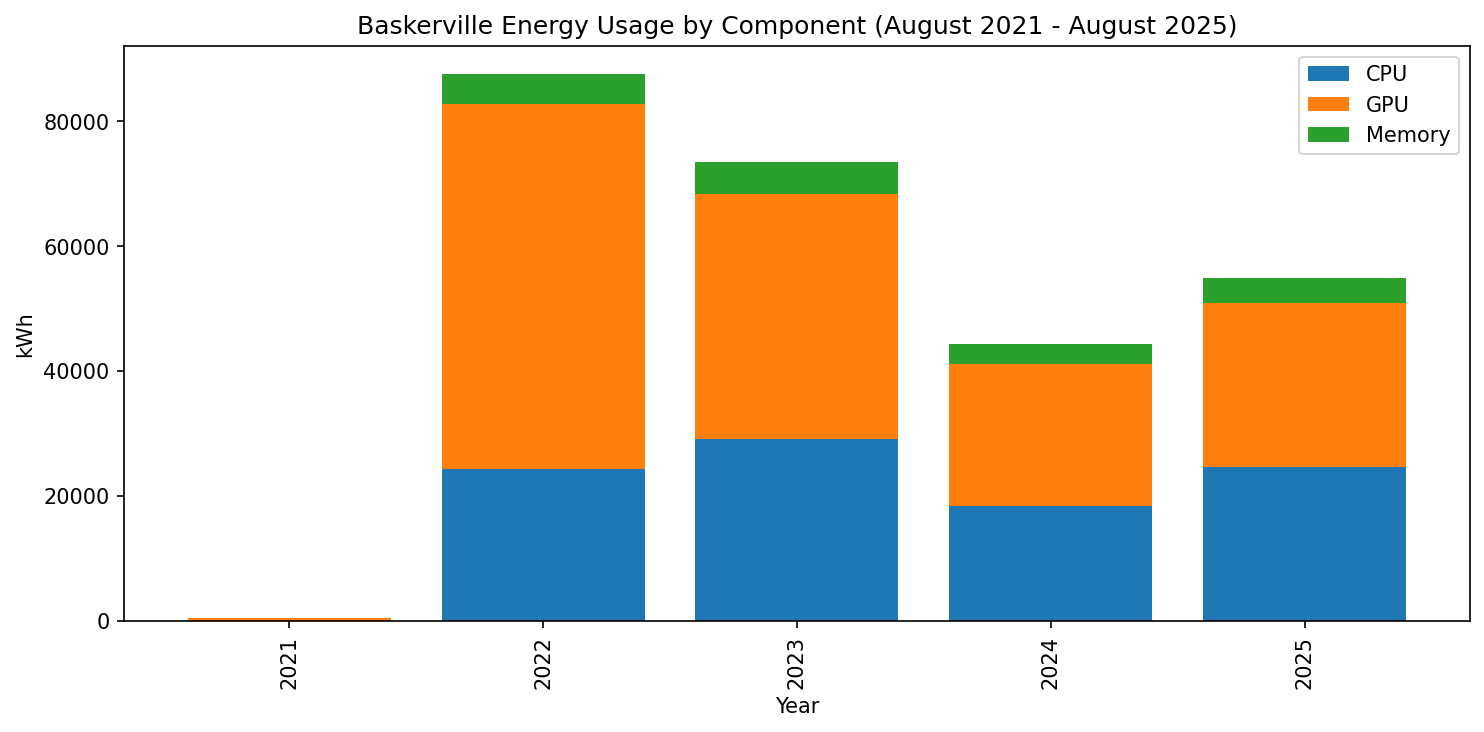
\includegraphics[width=0.75\linewidth]{baskerville_energy_per_component.png}
    \caption{Baskerville energy usage per year, broken down by component (August 2021--August 2025)}
    \label{fig:baskerville_energy}
\end{figure}

As per Equation \eqref{eq:emission1}, energy values per job are multiplied by carbon intensity at runtime to calculate carbon emissions. 
Two approaches to this are: using the carbon intensity of the University of Birmingham's CHP plant (\gcookwh{300}), or, using the carbon intensity of the national grid. 
For the latter, since carbon intensity values fluctuate throughout the day and throughout the year, different averaging approaches yield different emissions values. 
Three approaches to averaging carbon intensity are: 1.~Taking a yearly average (for exmaple, in 2024 the UK average carbon intensity was \gcookwh{124}~\cite{average_ci_2024}); 2.~Taking a daily average using the Carbon Intensity API\footnote{\url{https://carbon-intensity.github.io/api-definitions/\#carbon-intensity-api-v2-0-0}}; and 3.~Taking an hourly average, again using the Carbon Intensity API.

The \texttt{run\_baskerville\_emissions} notebook\footnote{\url{https://github.com/rwood-97/turing_emissions/blob/main/run_baskerville_emissions.ipynb}} shows the results under each of these different approaches.
Using the CHP plant approach, the Turing's operational emissions over its entire use of Baskerville were \qty[qualifier-mode=combine]{89.2}{\tonne\of{\cooe}} and its operational emissions in the past year (September 2024--August 2025) were \tcooe{25.0}. 
Using the national grid approach, with a yearly average carbon intensity of \gcookwh{124}, the Turing's operational emissions over its entire use of Baskerville were \tcooe{36.9} and its operational emissions in the past year (September 2024--August 2025) were \tcooe{10.3}. This is approximately \num{2.4} ($300/124$) times lower than using the CHP plant approach. This lower carbon intensity reflects the fact that the national grid draws from a mix of sources — including renewables and nuclear, which have near-zero carbon intensities — whereas the CHP plant runs purely on gas. 
Notably, even when using the national grid approach, our operational emissions from Baskerville usage are significantly higher than from our entire Azure usage (operational plus embodied emissions).

Using the national grid approach with daily average CIs, the Turing's operational emissions over its entire use of Baskerville were \tcooe{48.5} and its operational emissions in the past year were \tcooe{10.9}.
Using this approach, our overall emissions were higher but our emissions for the past year were lower.
These variations are due to a reduction in grid carbon intensity over time as more renewables are added to the national grid, meaning historical CIs were higher than \gcookwh{124} but this current year's average carbon intensity is lower.

A number of open source tools for measuring operational emissions from HPC are available on GitHub~\cite{greenalgorithms4hpc, grace_hpc}. {GRACE-HPC}, developed by Elliot Ayliffe and the Bristol Centre for SuperComputing (BriCS) team~\cite{grace_hpc}, is one example.
Generally, these tools use the slurm \texttt{sacct}\footnote{\url{https://slurm.schedmd.com/sacct.html}} command (or the non-slurm equivalent of this command if an alternative job scheduler is being used) to gather information about completed jobs and calculates their carbon emissions based on the carbon intensity at the job's run time. 
However, due to privacy restrictions, Baskerville users are only able to see information about their own jobs using \texttt{sacct}. 
This is true even for Turing admins and so instead of running GRACE-HPC directly on Baskerville, \texttt{sacct} data for the Turing's usage of Baskerville was kindly provided directly by the Baskerville team. 
The code was adapted to use this pre-saved data as input.\footnote{Specifically, to save time and reduce the number of API calls, some caching was added and the carbon intensity averaging adjusted to use hourly averages rather than exact carbon intensity values on a job-by-job basis. See pull requests \#1 (\url{https://github.com/Elliot-Ayliffe/GRACE-HPC/pull/1}), \#2 (\url{https://github.com/Elliot-Ayliffe/GRACE-HPC/pull/2}) and \#3 (\url{https://github.com/Elliot-Ayliffe/GRACE-HPC/pull/3}).}

Running GRACE-HPC on the provided data showed that the Turing's operational emissions were approximately \tcooe{11.2} from its usage of Baskerville in the past year (September 2024--August 2025).
Notably, this is around \qty{25}{\percent} higher than calculated using daily average CIs, though it is unclear where these differences arise.
This aligns with the numbers seen when using the daily averaging approach, showing that approximating with a daily average carbon intensity is a reasonable choice.

Figure \ref{fig:agg_hourly_run_time_baskerville_vs_ci} shows how the Turing's usage of Baskerville and the UK average carbon intensity vary throughout the day. From this, we see that on average the Turing has the highest number of jobs running between 11 am and 5 pm. Interestingly, when compared against the UK average carbon intensity, we see that our jobs are generally being run when carbon intensity is lowest.  

\begin{figure}[ht!]
    \centering
    \includegraphics[width=0.75\linewidth]{uk_ci_vs_usage.png}
    \caption{UK average carbon intensity and average number of Baskerville jobs running at each hour of the day (September 2024--August 2025).}
    \label{fig:agg_hourly_run_time_baskerville_vs_ci}
\end{figure}


GRACE-HPC also highlights other data from our Baskerville usage.
For example, the Turing ran \num{48099}
  jobs over the course of the last year, summing to \qty{138073}{\GPUh}. 
  However, around half (\qty{48.9}{\percent}) of those finished with a non-zero exit code. This indicates that these jobs did not run to completion. This could mean that jobs were interrupted due to an error or due to time constraints and therefore there is potential for lost results and wasted energy. According to GRACE-HPC, these jobs account for approximately \tcooe{7.1}---over half of the Turing's Baskerville emissions. Reducing the number of these jobs would significantly reduce our operational emissions from HPC use. This could be achieved by offering more training for new HPC users, guidance on best practices when submitting jobs to HPC and raising awareness of the emissions from failed jobs.

A full comparison between the four methods is shown in Table \ref{tab:op_emissions_comparison}. Clearly, the biggest influence on the operational emissions from our Baskerville usage is the provider of the electricity with less influence coming from the averaging method. Since the source of electricity for Baskerville HPC is a CHP plant, these numbers from the CHP plant approach are likely the best estimate of the four methods. Due to the errors in the energy estimates (mentioned above) and variations in the carbon intensity values, these operational emissions values should still only be taken as rough estimates.

\begin{table}[ht!]
    \centering
\caption{Comparison of the different methods for calculating operational emission from HPC}
\label{tab:op_emissions_comparison}
    \begin{tabular}{rrrr}\toprule
        Approach&  Averaging method&  \shortstack{All time\\emissions / t\cooe}& \shortstack{Year to date\\/ t\cooe}\\\midrule
         CHP plant &  Yearly&  89.2& 25.0\\
         National Grid&  Yearly&  36.9& 10.3\\
         National Grid&  Daily&  48.5& 10.9\\
         National Grid&  Hourly&  N/A& 11.2\\ \bottomrule
    \end{tabular}
    
    
\end{table}

\subsubsection{Emissions rate}

Since we don't necessarily want to reduce our usage of HPC, it's useful instead to think of emissions as a rate per functional unit.
For example, per \unit{GPUh}, per useful output or, for AI workloads, per token.
In the past year, the Turing ran jobs summing to \qty{138073}{\GPUh} and so our emissions rate is \qty[qualifier-mode=combine,per-mode=symbol]{81.3}{\gram\of{\cooe}\per\GPUh} (using the \unit{GPUh} and emissions values reported by GRACE-HPC).
Methods of improving this rate would include making code more efficient by reducing idle times or using more efficient algorithms, ensuring requested resources are correct for the workload (\eg, ensuring the optimal number of GPUs/nodes/memory) and running jobs at times where carbon intensity is lower (also known as carbon aware scheduling). For the latter, this is only a viable approach if a) Baskerville GPU's are being used at less than \qty{100}{\percent} capacity and b) it was a system-wide approach, i.e. there are no rebound effects.
A similar approach could be taken for AI workloads using rate per token. 

\subsubsection{Embodied emissions}

Recent work focused on estimating the embodied emissions of HPCs from the Top500 list\footnote{\url{https://top500.org/lists/top500/}}~\cite{Rao_2025} estimated Baskerville's embodied emissions to be \tcooe{381}. This value was calculated using EasyC~\cite{easyc}, a tool which estimates embodied carbon emissions based on a only few simple parameters – the number of compute units, storage capacity and memory capacity.

To verify this number, we can compare against other HPCs for which in-depth embodied emissions analyses have been undertaken. For example, the embodied emissions from Isambard-AI (Phase 2), a GPU-based HPC, is estimated to be \tcooe{8184}~\cite{isambard-ai_emissions}. Isambard-AI (Phase 2) is made up of \num{1320} nodes with GH200 chips. Each GH200 chip has one Grace CPU and one H100 GPU. There are four GH200 chips per node and \num{72} cores per GPU. Isambard-AI also has \num{1056} \qty{30.72}{\tera\byte} NVMe SSDs.~\cite{isambard-ai_specs} In comparison, the Baskerville system is made up of \num{48} nodes with A100 GPUs and two nodes with H100 GPUs. For both A100 and H100 nodes, there are four GPUs per node and \num{36} cores per GPU. Baskerville also has \num{48} \qty{7.68}{\tera\byte} SSDs. From these system specifications, we see Isambard-AI has $26\times$ more compute nodes than Baskerville. A naive estimate for the embodied emissions of Baskerville would therefore be around \tcooe{310} ($8184/26$). However, this does not account for the different GPUs types, number of CPUs per node or SSD capacities. Nevertheless, this supports the idea that embodied emissions for Baskerville HPC should be on the order of \tcooe{300}. 

Embodied emissions can be converted to embodied emissions per unit time such that embodied emissions can be apportioned to the different users of these HPC systems based upon their usage. For Isambard-AI, using an estimated 6 year service lifetime, embodied emissions are estimated to be \qty[qualifier-mode=combine]{0.114}{\kilogram\of{\cooe}} per node hour~\cite{isambard-ai_emissions, archer2_sustainability}.
Since Baskerville has been running since 2021 and is due to be shut down in 2026, its service lifetime is 5 years. 
This gives an estimated embodied emissions per unit time of \qty[qualifier-mode=combine]{0.174}{\kilogram\of{\cooe}} per node hour or \qty[qualifier-mode=combine]{0.043}{\kilogram\of{\cooe}\per\GPUh}.
Given our usage over the past year of \qty{138073}{\GPUh}, the Turing's share of embodied emissions from our Baskerville usage is \tcooe{6} in the past year.
Comparing this against the values in Table~\ref{tab:op_emissions_comparison}, this suggests that over the past year operational emissions outweighed embodied emissions for Baskerville HPC. This means that pushing for Baskerville to be powered by renewable electricity, or moving to a greener HPC, would be the most effective method of reducing our emissions from compute. Notably, since embodied emissions are fixed at the point of manufacture, embodied emissions generally dominate over operational emissions in newer HPCs. Thus, maximising HPC utilisation is the most carbon-efficient way to spread those costs across useful work.

\section{GitHub Actions}
\label{sec:github}

Since GitHub uses Azure virtual machines (VMs) to run GitHub Actions workflows, and we know that Azure uses renewable electricity with a carbon intensity of zero, the most likely value for the Turing's operational emissions from GitHub actions is zero. Our embodied emissions are more difficult to estimate, but are likely to be low, since GitHub actions uses small VMs with only a few CPUs. Optimising our use of GitHub actions is therefore not likely to impact our overall emissions from compute.

\subsection{Market-based emissions}

For sake of argument, it is possible to calculate the Turing's emissions from GitHub Actions using the market-based approach. The Turing's GitHub organisation\footnote{\url{https://github.com/alan-turing-institute}} ran \num{3340} hours of GitHub Actions in the past six months (March 2025--September 2025). To estimate the operation emissions from this work, we must know a) the energy consumption and b) the carbon intensity of the energy consumed.

GitHub provide some information about the default runners used when a
GitHub Actions workflow is triggered, including information about the
number of CPUs and RAM on the VM~\cite{github_runners_info}. This helps
us understand what compute resources are being used and thus estimate
their energy consumption.  To understand the carbon intensity of the energy consumed,
we need to know where this energy is coming from. I created a support
request to GitHub to ask about the location of these runners and got the
following response: ``Standard and larger GitHub-hosted runners are all
hosted in North America (primarily in the United States, and
occasionally Canada).'' Together, this information can be used to work
out the approximate operational emissions from the Turing's use of
GitHub actions using the Green Algorithms
calculator~\cite{green_algorithms}.

In the previous six months, a rough estimate for our operational emissions related to GitHub actions runners is \qty[qualifier-mode=combine]{50}{\kilogram\of{\cooe}}.
This was calculated using the Green Algorithms calculator and the following settings: \num{3340} hours of runtime, four CPUs, \qty{7}{\giga\byte} memory and setting the Azure region as North Central~US.
Assuming this value is representative, this equates to just \qty[qualifier-mode=combine]{100}{\kilogram\of{\cooe}} for the year - negligible compared to our Azure and HPC emissions and confirms that optimising GitHub Actions usage is unlikely to significantly affect our overall compute-related emissions.

\section{Conclusion}
\label{sec:conclusion}

This report explores three different sources of computing emissions from the Turing: Microsoft Azure, HPC and GitHub Actions. The Turing's emissions from these compute resources are summarised in Table~\ref{tab:summary_table}. In total, we were responsible for around \tcooe{34} emissions from compute in the past year. This is equivalent to just under seven times the average UK per-capita emissions, around 35 passengers on a transatlantic flight to New York, or over 100 passengers on a short-haul flight to Madrid. More than anything, this demonstrates the huge emissions impact of flying.

Notably, the majority of the Turing's compute emissions came from Baskerville HPC, a GPU-based machine where the bulk of our workloads are AI-focused. This highlights the large impact of AI's emissions compared to other computing workloads and suggests contributing to research into greener AI technologies would be an effective route to reducing the Turing's emissions whilst also having a wider impact.

Reducing emissions from Baskerville is currently the largest opportunity for reducing our emissions, the easiest way of doing this would be to encourage the Baskerville team to put Baskerville on a renewable electricity tariff. 
An alternative approach, especially in light of Baskerville's end of life in 2026, would be to encourage Turing projects to move to a greener HPC. Other potential avenues for reducing the Turing's emissions from Baskerville usage include reducing the number of failed jobs --- for example, by providing more training or guidance for HPC users --- and improving the efficiency of jobs by optimising the compute resources requested or using more energy efficient algorithms.

Other potential sources of emissions not covered in this report due to lack of data include other UK HPCs which the Turing makes use of (Isambard-AI and Dawn), Turing-owned hardware (laptops, commercial GPUs and Pi's) and collaborators' hardware.

% \bibliography{bibliography}{}
% \bibliographystyle{plain}
\printbibliography

\end{document}


